
\section{Experimental Results}

\begin{figure}[ht]
  \centering
  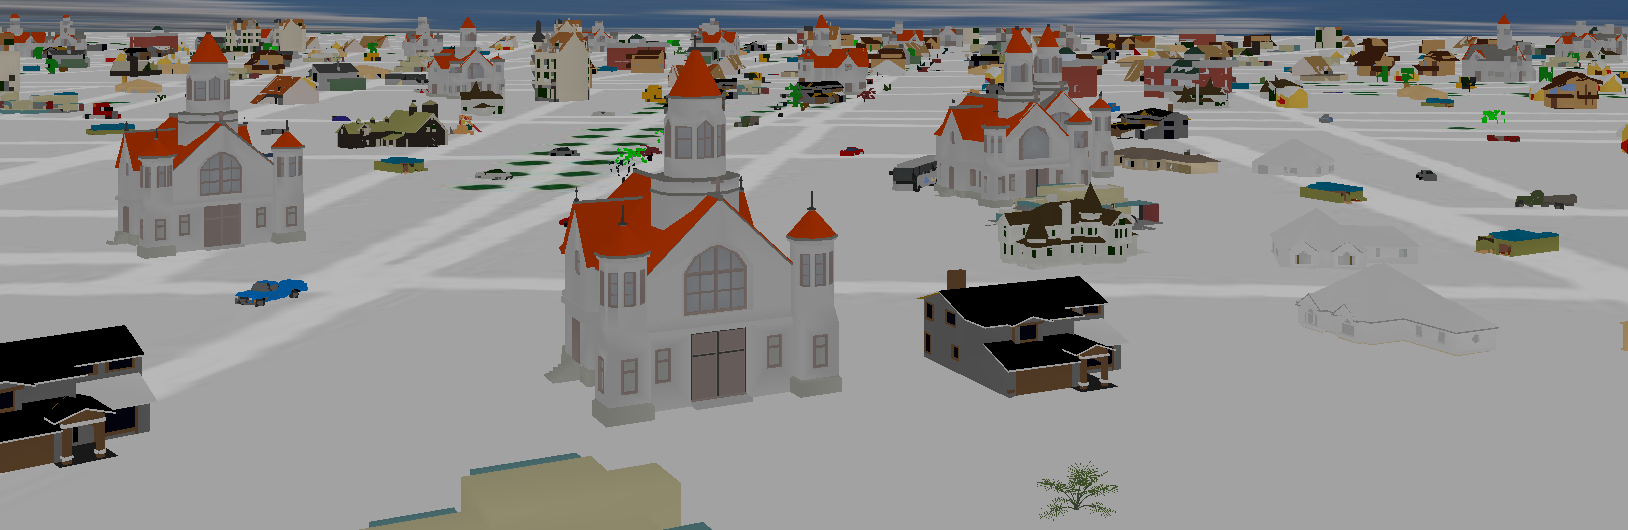
\includegraphics[width=\columnwidth]{city.png}
  \caption{City model: 110 million triangles, 6 GB }
  \label{fig:model1}
\end{figure}

\begin{figure}[ht]
  \centering
  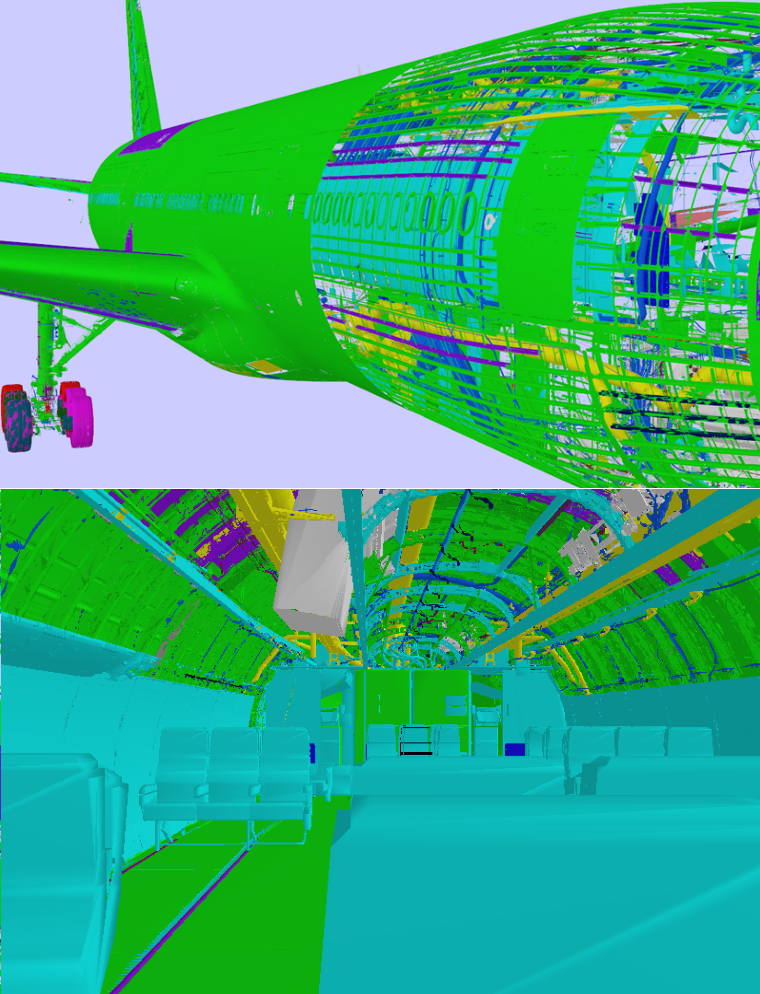
\includegraphics[width=\columnwidth]{BoeingModel.pdf}
  \caption{Boeing model: 350 million triangles, 20 GB. Overview of model (top) and model detail (bottom)}
  \label{fig:model2}
\end{figure}

\begin{figure}[ht]
  \centering
  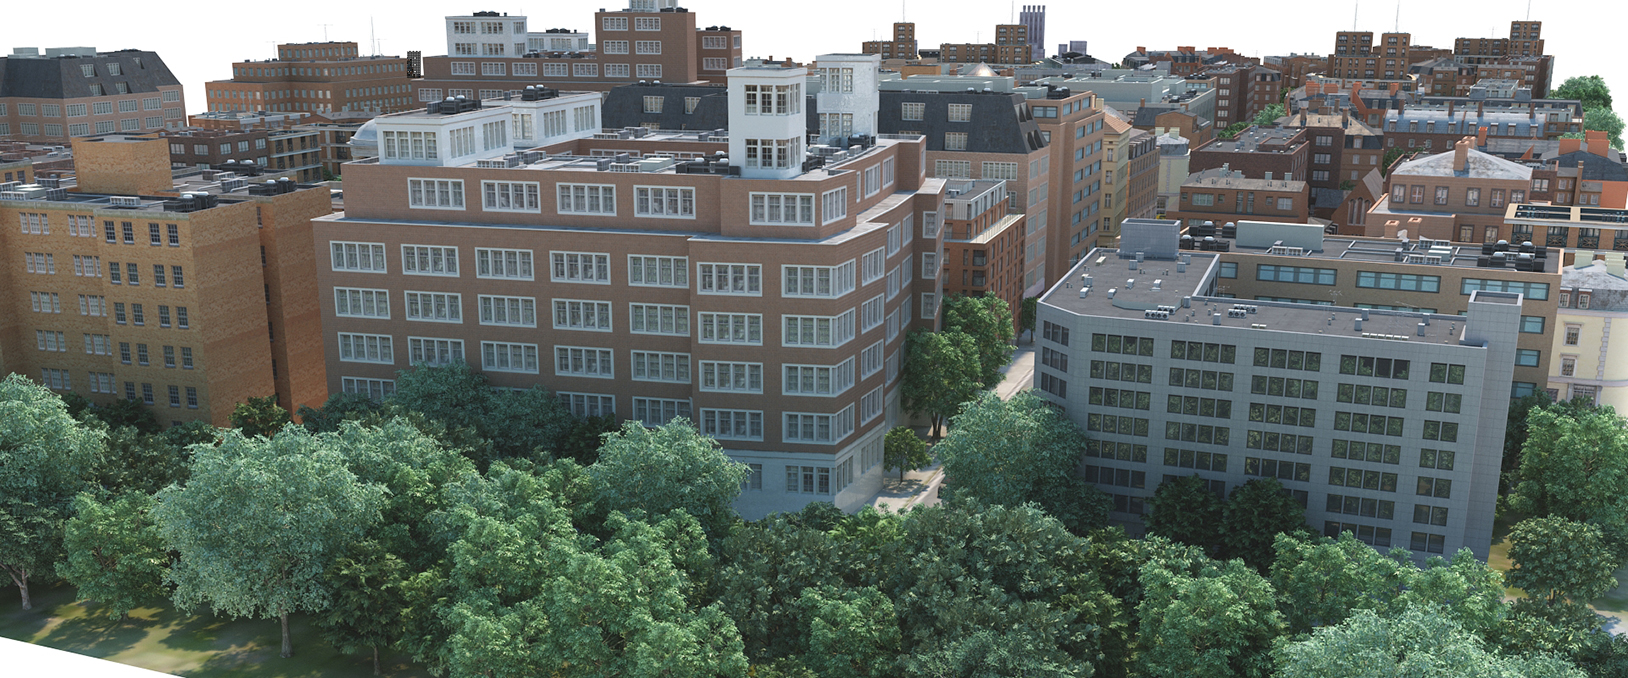
\includegraphics[width=\columnwidth]{densecity.jpg}
  \caption{Urban model: 100 million triangles, 12 GB }
  \label{fig:model3}
\end{figure}


\textbf{Experiment context:}
In order to implement our algorithm, we used a workstation that is a Dell T5400 PC with Intel (R) Core (TM) 2 Quad and $8GB$ main memory. The hard drive is a 1TB Seagate Barracuda with 7200 RPM and the graphics card is an nVIDIA Geforce GTX 260 with 896 MB GPU memory. The data rate of the hard drive is $120$ MB/s and the seek time is a minimum of $2$ ms per disk seek.\\
\\
\textbf{Benchmarks:}
We use three models to perform our experiments, each model represents a use
case or scenario. The City model (Figure \ref{fig:model1}) is a regular model
that can be used in a navigation simulation application or virtual reality
walkthough. The Boeing model (Figure \ref{fig:model2}), on the other hand,
represents scientific or engineering visualization applications. The Urban
model (Figure \ref{fig:model3}) has texture attached to it, which is commonly
used in games. By comparing performance of cache-oblivious layout without
redundancy~\cite{cacheobliviouslayout} to our method using redundancy on these three models, our goal
is to show that the redundancy based approach can achieve more stable and generally
better performance on different real time applications. \\
\\ To apply our method on these large-scale models, we had to find a proper set
of access requirements. In general, that question is deep enough that it can be
discussed as a separate research topic. Here, however, we had good performance
using only simple schemes for creating access requirements. Each model ended up
having a separate scheme. Nonetheless, an access requirement represents a set
of data that is highly likely to be accessed together. \\
\\
For the City model, a 2D grid is used to divide the space into square cells. For each pair of adjacent cells, the difference of the data is considered as an access requirement\YOON{Difference is access requirement? Odd. I guess that you are using pairs as accesses, and the diff. means their length in the 1 D layout?}. By propagating this rule, access requirements are created, and the number of them is determined by the resolution of the grid. \YOON{How many access requirement do you have in the end? For each cell, do you create an access requirement? Also, explain why you adopt this way of creating access requirement.} \\
\\
For the Boeing model, the predefined objects are used as a conceptual level to create access requirements. Samples of view positions are distributed across the model. For each sample, four fixed directions and four random directions are considered. Objects visible from this position in any one of these eight directions are added to access requirement for this specific sample. The density of these samples depends on the complexity of local occulders to reduce load of each access requirement, i.e. more samples are distributed to places with more complex geometry. \\
\\
The Urban model is different from the previous two in a way that it involves textures. Building heavy redundancy of textures increases the total size of the dataset significantly, while keeping textures away from redundancy leads to inevitable long seek time, which is completely against the philosophy of this work. To solve this problem, we applied a spatial Lloyd’s clustering\YOON{We need a citation for this.} on objects. By moving centers of clusters, we look for a solution such that each cluster involves almost same amount of texture data. Between clusters, textures can be redundantly stored, but within each cluster, texture data are stored uniquely. In this way, each cluster is used as an access requirement.  \\
\YOON{Mention how long does it take to compute the redundancy layout for each model.}
\\
\textbf{Results:}
Figure \ref{fig:resultall} shows the results of delays caused by fetching data on the experimental models we used. We compare the results of a cache-oblivious layout without redundancy and one with redundancy. For the layout with redundancy, we set the redundancy factor equal to 4.2. This factor was chosen because as can be seen in Figure \ref{fig:statistic}, it had considerably better performance than lower redundancy factors and did not have significantly worse performance than higher redundancy factors. A factor of 4.2 is also still practical, as the largest model we tested, the Boeing model, becomes 84 GB which is still acceptable given the large capacity of modern secondary storage devices.\\
\\
It is clear that the performance of the layout with redundancy has generally shorter delays than the cache-oblivious layout without redundancy. As can be observed from the results, although the layout with redundancy does not eliminate delays for most of sample points on the walkthrough path, it reduces delays to a small range and keeps the performance more consistent. This is the benefit we get from using our algorithm which adds redundancy. Since the algorithm tends to eliminate seeks with longer seek time first, in practice the larger delays are avoided.
\begin{figure}[ht]
\centering
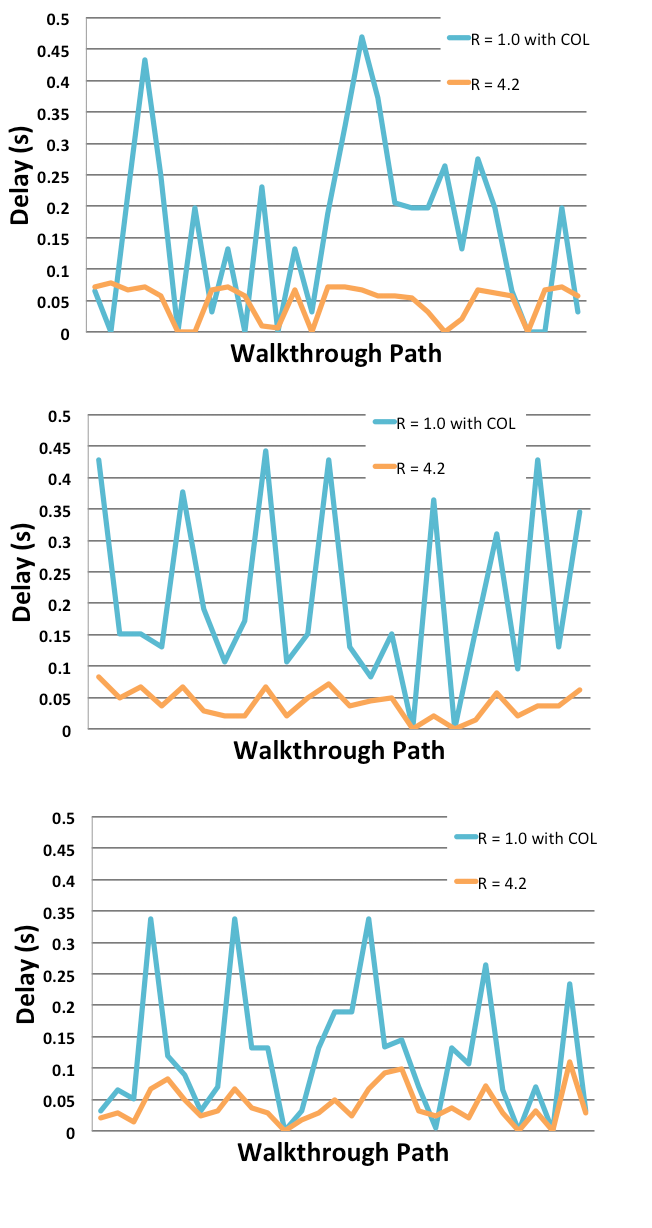
\includegraphics[width=\columnwidth]
{resultall.png}
  \caption{Statistics of delays caused by the fetching processes for the City model (top), the Boeing model (center), and
the Urban model (bottom), with and without redundancy. }
  \label{fig:resultall}
\end{figure} 

\begin{figure}[ht]
\centering
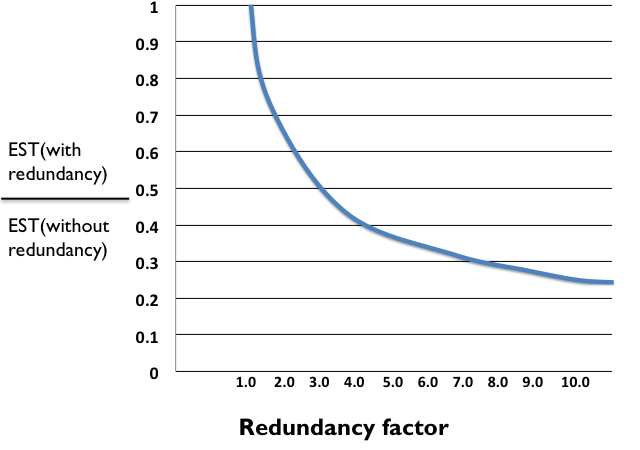
\includegraphics[width=\columnwidth]{statistic.png}
  \caption{Plot of the ratio of the EST of layout with redundancy over the EST of cache-oblivious mesh layout without redundancy. }
  \label{fig:statistic}
\end{figure} 

There is another major benefit to our approach when compared to \cite{optimizingredundancy} in which the user does not have any control over the final redundancy factor. Since each time we duplicate one data unit, we can halt it when the redundancy factor reaches a certain threshold. This helps us create a data layout with arbitrary redundancy factor without worrying about exceeding the capacity of secondary storage devices. We use this fact to test different redundancy factors and see their results. In Figure \ref{fig:statistic}, we show the results of using layouts with redundancy factors that range from 1.0 to 10.0. The y-axis in this figure is the ratio of the estimated seek time (EST) of the layout with redundancy over the EST of the layout without redundancy. This value starts at 1.0 where redundancy factor is 1.0, meaning no redundancy, and decreases as redundancy factor goes larger. We can see that the rate of this decrement is not constant, and the benefits we gain at beginning are larger than the ones we get later. This implies that most of the performance improvement resides at the earlier phase of raising redundancy factor. This implies that it is worth to limit the redundancy factor used because after a certain point you are using much more secondary storage space without improving seek time by much. It also implies that our algorithm dramatically reduces seek time in practice by using only small redundancy factors. 

